% !TeX root = ../main.tex
% Add the above to each chapter to make compiling the PDF easier in some editors.

\chapter{Advanced quantization approaches}
\section{Shift to INT-based mixed-precision}
\subsection{Shortcomings of previous approaches}
\begin{figure}
\centering
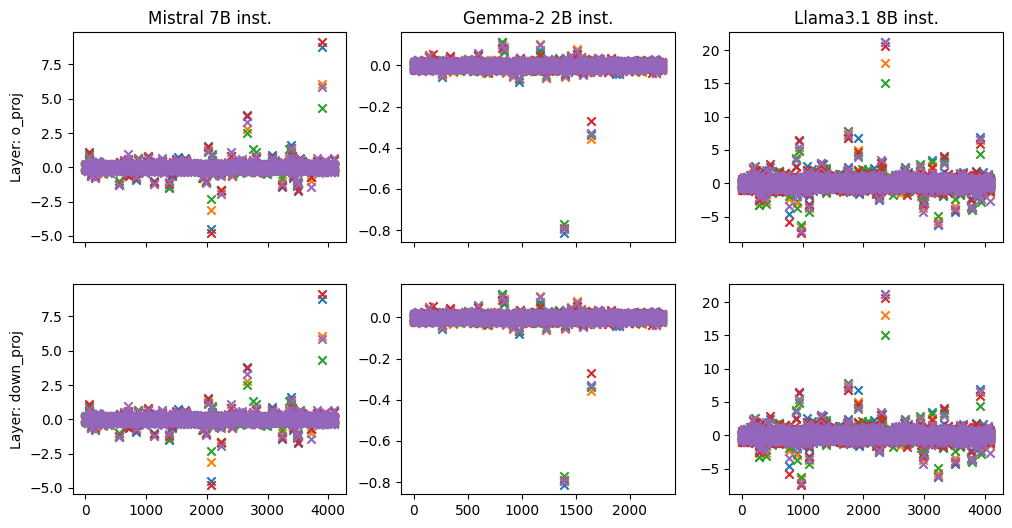
\includegraphics[width=0.5\textwidth]{figures/plot_outlier_channels}
\caption{Outliers within a single layer.}
% Activation shards from the row-wise TP layers are being synchronized using the all\_gather collective op across devices before reduction, which we propose to compress as shown in Figure.}
\label{fig:plot_outlier_channels}
\end{figure}

\begin{itemize}
	\item all layers are treated in the same way, although the activations differ greatly
	\item plot (\ref{fig:plot_outlier_channels}) (last layer of each model): show we have outlier channels (also according to literature); outlier channels are static
    \item should treat outlier channels differently
\end{itemize}

%\subsection{Outlier channels are static}
%\begin{itemize}
%	\item introduce outlier metric
%	\item show we have a high overlap, proof finding above (outliers are static)
%\end{itemize}

\subsection{Method}
\begin{itemize}
    \item saw that INT quantization leads the best TTFT improvements, but aren't great regarding accuracy

    \item idea: quantize inlier- and outlier-channels differently
    \item we know outlier channels are static: identify offline outlier channels, which will be kept in higher precision (quantized using less aggressive scheme)
    \item remaining channels are quantized to lower bits/value
\end{itemize}

%\subsection{(Runtime compared to single-precision INT)}
%takeaway: INT-based mixed precision is only slightly slower

\subsection{How to identify outlier channels?}
\begin{itemize}
    \item different literature methods: Atom and LLM.int8(), both are quantization-agnostic
    \item we consider more methods, which track the quantization error
    \item won't do an experiment here, but instead consider all these methods for further experiments
\end{itemize} 

\section{Naive approach}
like Atom etc: keep fixed \% of channels in high precision
try different low-precision bits

\begin{itemize}
	\item try different low-precision bits
	\item compare zero-shifting with non-zero-shifting
	\item show different ordering approaches
	\item determine how to pick best approach for some model, i.e. take approach with best bits/value which achieves perplexity below some threshold; then evaluate on test set
\end{itemize}


\section{Local error based outlier channel selection}
\subsection{Motivation}
\begin{figure}
\centering
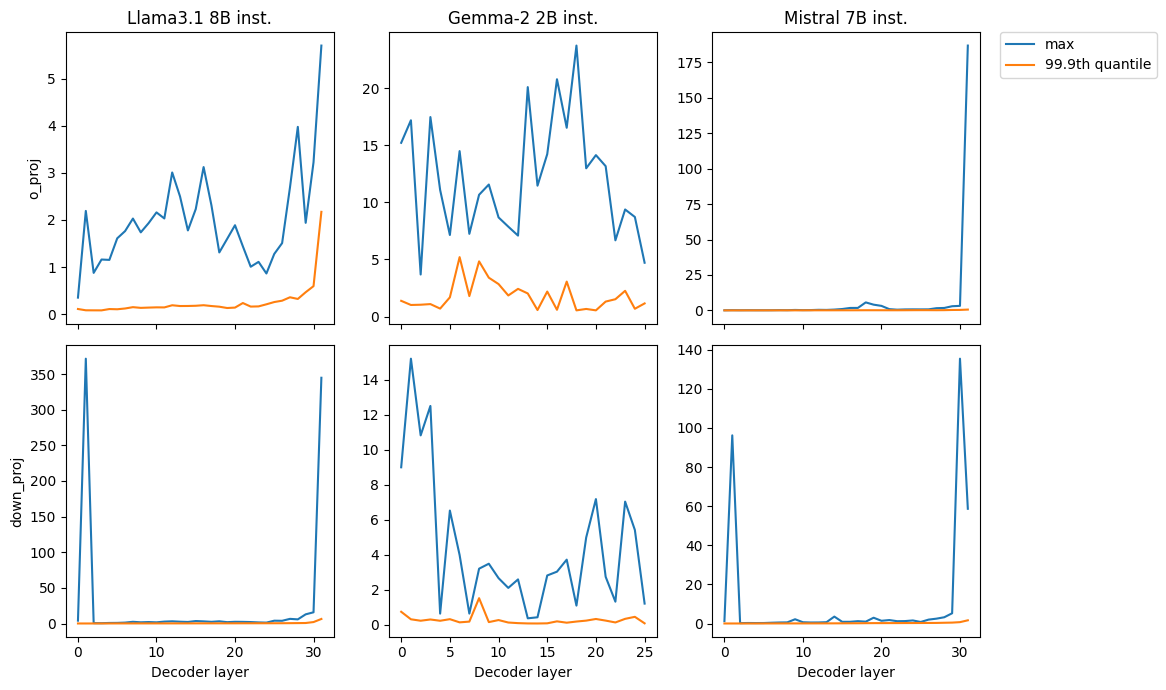
\includegraphics[width=0.5\textwidth]{figures/plot_outlier_layers}
\caption{Outliers within a single layer.}
% Activation shards from the row-wise TP layers are being synchronized using the all\_gather collective op across devices before reduction, which we propose to compress as shown in Figure.}
\label{fig:plot_outlier_layers}
\end{figure}

\begin{itemize}
	\item plot: (\ref{fig:plot_outlier_layers}) using argmax(channel), show percentage of ourlier channels per layer
    \item layers contain very different amounts of outlier channels
    \item idea: automatically determine \% of outlier channels layer-wise
\end{itemize}


\section{Automatic mixed precision parametrization}

\section{Profiling}
\begin{itemize}
	\item comparison of different mixed approaches with SoTA -> they are outperformed
\end{itemize}
